\documentclass[11pt,a4paper]{report} 

\usepackage[utf8]{inputenc} 
\usepackage[norsk]{babel} 
\usepackage{lipsum,paralist}
\usepackage{enumitem}
\usepackage{graphicx}
\usepackage{float}
\usepackage{chngpage}
\usepackage{calc}


\begin{document}
\title{
\LARGE
Forprosjektrapport \\
\vspace{2cm}
Utvikling av nettsted for Sirkus Media \\
\vspace{2cm}
\Huge
B019-G13
}
\author{
\LARGE 
Bereket Goitom Adhanom \\
\LARGE 
Bjørnar Hagen \\
\LARGE 
Line Sharina Aamodt Hagen
}
\maketitle

\section*{Prosjektgruppen}

Deltagerne i prosjektgruppen ble raskt kjent på det obligatoriske sommerkurset til Y-veien på dataingeniørstudiet. Siden den gang har vi samarbeidet på gruppeoppgaver underveis i studiet. Alle deltagerne har alltid samarbeidet godt, og dette var en viktig faktor når vi skulle danne en gruppe for bacheloren. 

\subsection*{Om Bereket}
Gikk på IKT-servicefag på  videregående og var deretter lærling hos IT-avdelingen til Rana kommune. Etter bestått fagbrev begynte jeg på Høgskolen i Østfold på dataingeniørstudiet Y-vei.

Er interessert å jobbe med teknologier som HTML, CSS, PHP og JavaScript.

\subsection*{Om Bjørnar}
Tok fagbrev som IKT-servicemedarbeider hos Optimale Systemer AS i Larvik etter 2 år som lærling. Dette etter å ha fullført IKT-linja hos Sandefjord videregående skole. Deretter gikk det videre til Høgskolen i Østfold, og startet da på Y-veien for dataingeniørstudiet.

Jobber nå som daglig leder hos Datahjelpen AS, hvor arbeidsoppgavene innebærer utvikling som full-stack og en del DevOps. Liker å jobbe med teknologier som HTML, CSS, JavaScript, Node, React, PHP og Linux.

\subsection*{Om Line}
Gikk IKT-servicefag på Sandefjord videregående skole. Var etter dette lærling hos Vestfold Fylkeskommune der jeg tok fagbrev og dermed ble utdannet IKT-servicemedarbeider. Startet deretter på Y-veien på dataingeniørstudiet ved Høgskolen i Østfold. 

Jobber nå som front-end utvikler hos Datahjelpen AS og liker best å jobbe med teknologier som HTML, CSS, JavaScript og PHP.

\section*{Oppdragsgiver}

Sirkus Media ble stiftet i 2010 av Hans-Christian Hymer og er et teknologi-, data- og analyseselskap som leverer innovative løsninger for digital markedsføring. Deres kunder er små og store bedrifter i hele Norge som ønsker å få økt salg og lønnsomhet. 

Ved hjelp av deres egenutviklede løsning jobber de med å skaffe konkrete kundehenvendelser til sine kunder. Løsningen når direkte ut til kjøpsklare kunder. Dette innebærer at de utelukkende markedsfører mot personer som, basert på nettadferd, vet at med stor sannsynlighet er på utkikk etter produkter eller tjenester som selskapet tilbyr.

Sirkus Media har i dag 2 ansatte og hadde i 2017 en omsetning på 6.4 millioner.

Vår kontaktperson hos oppdragsgiver er Hans-Christian Hymer som både er grunnlegger og daglig leder av Sirkus Media. 

\section*{Oppdraget}

Bakgrunnen for dette oppdraget er at Sirkus Media ønsker å forbedre deres profil på nett, slik at potensielle kunder får en bedre forståelse av deres produkter og tjenester og tar kontakt gjennom nettstedet. Dette er viktig for oppdragsgiver ettersom dagens nettsted har store mangler og ikke inneholder nok informasjon om hva Sirkus Media tilbyr. Sirkus Media har derfor et stort behov for utvikling av en ny nettside. 

Nettstedet skal inkludere en løsning for skjemahenvendelser, beskrive Sirkus Media sitt produkt, hva de tilbyr, resultater de kan vise til og omtale fra eksisterende kunder.
I tillegg skal nettstedet inneholde informasjon angående deres prosess, live chat og kart integrert med Google Maps. Oppdragsgiver ønsker også å ha muligheten til å logge inn på nettstedet og selv kunne oppdatere innhold.

\subsection*{Formål}

\begin{compactitem}
\item [{\bf Hovedmål}] Forbedre Sirkus Media sin profil på nett, slik at potensielle kunder får en bedre forståelse av deres produkter og tjenester og dermed tar kontakt gjennom deres nettsted. På et overordnet plan vil dette bidra til å øke omsetningen til oppdragsgiver.
\begin{compactitem}
\item [{\bf  Delmål 1} ] Generere mer trafikk, som fører til at flere kunder tar kontakt med bedriften. 
\item [{\bf  Delmål 2} ] Måle trafikken på nettstedet, slik at man ser hva som fungerer og deretter kan tilpasse informasjonen til brukerne som besøker siden.
\end{compactitem}
\end{compactitem}

\subsection*{Leveranser}

Følgende dokumenter må leveres:
\begin{itemize}
\item Prosjekt og gruppekontrakt
\item Gruppenettsted
\item Forprosjektrapport
\item Første versjon av hoveddokument
\item Andre versjon av hoveddokument
\item Hoveddokument med vedlegg
\item Prosjektplakat
\item Presentasjon
\end{itemize}
I tillegg vil disse konkrete resultatene bli opprettet i løpet av dette prosjektet:
\begin{itemize}
\item Analyse av gammelt nettsted
\item Analyse av konkurrenter
\item Analyse av verktøy
\item Visuell profil og designsystem
\item Prototype og mockups av nytt nettsted
\item Database og modeller
\item Nettsted
\item Analyse av nytt nettsted
\item Sitemap
\item Brukerveiledninger
\end{itemize}

\subsection*{Metode}
Hovedmålet er å forbedre Sirkus Media sin nettprofil. Dette løser vi med å analysere dagens nettside og kartlegger hva som er bra og dårlig. Deretter går vi videre til å analysere konkurrentene sine nettsider og ser hvordan deres løsninger ser ut. 

Det første delmålet er å generere mer trafikk til nettsiden. Da må vi å lage et attraktivt nettsted som følger beste praksis for god søkemotoroptimalisering, semantikk og universell utforming. 

For å oppnå delmålet om måling av trafikk på nettstedet må vi benytte oss av verktøy som Google Analytics. 

Mockups oppnår vi ved å hente inspirasjon fra lignende nettsider og deretter lager et forslag på design til nettstedet.

Database og modeller løser vi ved å først tegne og deretter forbedre databasen ved hjelp av penn og papir. 

\section*{Prosjektplan}

Prosjektet består av en rekke aktiviteter med tidsfrister. Deltageren som er ansvarlig for oppgaven sørger for levering til avtalt tid. Ved eventuell forsinkelse må deltageren informere resten av gruppen om dette. Aktivitetene er satt opp i prioritert rekkefølge.

\smallskip

\newcounter{aktivitetTeller}
\setcounter{aktivitetTeller}{1}

\begin{compactdesc}
    \item [Aktivitet \arabic{aktivitetTeller}:] Første møte med oppdragsgiver
	\begin{compactitem}
	\item Start: 22.11.2018
	\item Slutt: 22.11.2018
	\item Bemanning: Hele gruppen
	\item Beskrivelse: Danner grunnlaget for prosjektet. Overordnet informasjon om oppdraget.
	\end{compactitem}
	\addtocounter{aktivitetTeller}{1}
	
	\item [Aktivitet \arabic{aktivitetTeller}:] Gruppenettsted
	\begin{compactitem} 
	\item Start: 18.12.2018
	\item Slutt: 08.01.2019
	\item Bemanning: Hele gruppen
	\item Ansvarlig: Bjørnar
	\item Leveranse: Nettsted
	\item Beskrivelse: Hjemmesiden skal inneholde kontaktinformasjon for deltagerne og en beskrivelse av prosjektet. Etterhvert skal alle dokumenter, media, og kildekode gjøres tilgjengelig.
	\addtocounter{aktivitetTeller}{1}
	\end{compactitem}
	
	\item [Aktivitet \arabic{aktivitetTeller}:] Forprosjektrapport
	\begin{compactitem}
	\item Start: 08.01.2019
	\item Slutt: 18.01.2019
	\item Bemanning: Hele gruppen
	\item Ansvarlig: Line
	\item Leveranse: Rapport
	\item Beskrivelse: Fastsetter formålet for prosjektet, hva gruppen skal levere og hvordan prosjektet skal utføres.
	\addtocounter{aktivitetTeller}{1}
	\end{compactitem}
	
	\item [Aktivitet \arabic{aktivitetTeller}:] Andre møte med oppdragsgiver
	\begin{compactitem}
	\item Start: 16.01.2019
	\item Slutt: 16.01.2019
	\item Bemanning: Hele gruppen
	\item Beskrivelse: Konkret informasjon om oppdraget og hva nettstedet skal innholde.
	\addtocounter{aktivitetTeller}{1}
	\end{compactitem}
	
	\item [Aktivitet \arabic{aktivitetTeller}:] Analysere nåværende nettsted
	\begin{compactitem}
	\item Start: 21.01.2019
	\item Slutt: 22.01.2019
	\item Bemanning: Bjørnar
	\item Leveranse: Rapport
	\item Beskrivelse: Dokumentasjon av analyse med forklaring av test-resultatene. Kjører nettstedet gjennom forskjellige verktøy og analyserer resultatene.
	\addtocounter{aktivitetTeller}{1}
	\end{compactitem}
	
	\item [Aktivitet \arabic{aktivitetTeller}:] Analysere konkurrenter
	\begin{compactitem}
	\item Start: 21.01.2019
	\item Slutt: 22.01.2019
	\item Bemanning: Line
	\item Leveranse: Rapport
	\item Beskrivelse: Finne konkurrentene sine nettsteder, se på løsningen deres og analysere dette.
	\addtocounter{aktivitetTeller}{1}
	\end{compactitem}
	
	\item [Aktivitet \arabic{aktivitetTeller}:] Analysere passende verktøy
	\begin{compactitem}
	\item Start: 21.01.2019
	\item Slutt: 27.01.2019
	\item Bemanning: Hele gruppen
	\item Ansvarlig: Bereket
	\item Leveranse: Rapport
	\item Beskrivelse: Informasjon om verktøyene vi har valgt, samt fordeler og ulemper med verktøyene. Begrunne hvorfor vi har tatt de valgene vi har gjort.
	\addtocounter{aktivitetTeller}{1}
	\end{compactitem}
	
	\item [Aktivitet \arabic{aktivitetTeller}:] Planlegge innhold
	\begin{compactitem}
	\item Start: 28.01.2019
	\item Slutt: 29.01.2019
	\item Bemanning: Hele gruppen
	\item Ansvarlig: Line
	\item Leveranse: Rapport
	\item Beskrivelse: Planlegge hvilke sider nettstedet skal bestå av og hva hver enkelt side skal inneholde.
	\addtocounter{aktivitetTeller}{1}
	\end{compactitem}
	
	\item [Aktivitet \arabic{aktivitetTeller}:] Design \& visuell profil
	\begin{compactitem}
	\item Start: 29.01.2019
	\item Slutt: 12.02.2019
	\item Bemanning: Bjørnar
	\item Leveranse: Profilhåndbok, designsystem, interaktiv prototype med mockups. 
	\item Beskrivelse: Profilhåndbok med informasjon om hvordan Sirkus Media kan/skal bruke logo, ikoner, farger og fonter. Interaktivt digitalt designsystem med gjenbrukbare React-komponenter som lar deg se og teste komponentene, samt kopiere koden for disse.
	\addtocounter{aktivitetTeller}{1}
	\end{compactitem}
	
	\item [Aktivitet \arabic{aktivitetTeller}:] Hoveddokument: Introduksjon
	\begin{compactitem}
	\item Start: 29.01.2019
	\item Slutt: 31.01.2019
	\item Bemanning: Line og Bereket
	\item Ansvarlig: Line
	\item Leveranse: Rapport
	\item Beskrivelse: Kort beskrivelse av gruppen, oppdragsgiver, oppdraget, formål, metode og leveranser
	\addtocounter{aktivitetTeller}{1}
	\end{compactitem}
	
	\item [Aktivitet \arabic{aktivitetTeller}:] Database 
	\begin{compactitem}
	\item Start: 29.01.2019
	\item Slutt: 31.01.2019
	\item Bemanning: Hele gruppen
	\item Ansvarlig: Bereket
	\item Leveranse: Modell/skisser og ferdig database
	\item Beskrivelse: Planlegge og skissere databasen ved hjelp av penn og papir. Deretter opprette den planlagte databasen gjennom phpMyAdmin og definere den i Laravel gjennom migration filer. 
	\addtocounter{aktivitetTeller}{1}
	\end{compactitem}
	
	\item [Aktivitet \arabic{aktivitetTeller}:] Første versjon av hoveddokument 
	\begin{compactitem}
	\item Start: 29.01.2019
	\item Slutt: 08.03.2019
	\item Bemanning: Hele gruppen
	\item Ansvarlig: Line
	\item Leveranse: Hoveddokument
	\item Beskrivelse: Nå skal struktur og layout skal være på plass. Tittelside og prosjektside, samt introduksjons- og analysedelen skal være ferdig og komplett. Ellers skal mest mulig av det vi har skrevet så langt være med. De "tomme" kapitlene skal inneholde en kort orientering om det kommende innholdet.
	\addtocounter{aktivitetTeller}{1}
	\end{compactitem}
	
	\item [Aktivitet \arabic{aktivitetTeller}:] Back-end
	\begin{compactitem}
	\item Start: 04.02.2019
	\item Slutt: 03.04.2019
	\item Bemanning: Bereket, Bjørnar
	\item Ansvarlig: Bereket
	\item Leveranse: REST-API med login
	\item Beskrivelse: Det skal lages et REST-API med Laravel. Dette gir brukere mulighet til å logge inn og administrere data og tilgang. Starter med å definere ruter og binder de opp til kontrollere. Kontrollerne henter ut mockup-data fra modeller i JSON. Dette er en stor fordel, som lar oss begynne med front-end samtidig. Man vil da bytte ut mockup-data med faktiske data ettersom koden blir ferdig.
	\addtocounter{aktivitetTeller}{1}
	\end{compactitem}
	
	\item [Aktivitet \arabic{aktivitetTeller}:] Front-end
	\begin{compactitem}
	\item Start: 04.02.2019
	\item Slutt: 03.04.2019
	\item Bemanning: Line, Bjørnar
	\item Ansvarlig: Line
	\item Leveranse: Nettsted
	\item Beskrivelse: Nettsted som kobler seg til REST-API'et via JavaScript biblioteket Axios og henter ut og viser dataene på en fin og oversiktlig måte. Nettstedet skal være optimalisert for søkemotorer ved å ha god semantikk og bruk av microdata. Nettsidene må være universelt utformet og følge de lover og regler som gjelder rundt dette. Designet på nettstedet skal være i tråd med Sirkus Media sin profil og benytte seg av designsystemet.
	\addtocounter{aktivitetTeller}{1}
	\end{compactitem}
	
	\item [Aktivitet \arabic{aktivitetTeller}:] DevOps
	\begin{compactitem}
	\item Start: 25.03.2019
	\item Slutt: 08.04.2019
	\item Bemanning: Bjørnar
	\item Leveranse: Server som kjører LEMP-stack'en.
	\item Beskrivelse: Sette opp en server med Linux (Ubuntu), Nginx, MariaDB, PHP og phpmyadmin. Det skal settes opp backup av både filer og database. En beta versjonen av nettstedet skal settes opp og kjøre på serveren, frem til ferdig produkt er klart.
	\addtocounter{aktivitetTeller}{1}
	\end{compactitem}
	
	\item [Aktivitet \arabic{aktivitetTeller}:] Brukertesting
	\begin{compactitem}
	\item Start: 09.04.2019
	\item Slutt: 15.04.2019
	\item Bemanning: Hele gruppen
	\item Ansvarlig: Line
	\item Leveranse: Dokumentasjon av brukertester
	\item Beskrivelse: Alle gruppedeltagere samt oppdragsgiver tester nettstedet og dets funksjonalitet. Testene skal dokumenteres. Feil som oppdages rettes. Rettingen blir gjennomført av deltageren som var ansvarlig for aktiviteten med feil.
	\addtocounter{aktivitetTeller}{1}
	\end{compactitem}
	
	\item [Aktivitet \arabic{aktivitetTeller}:] Andre versjon av hoveddokument 
	\begin{compactitem}
	\item Start: 11.03.2019
	\item Slutt: 23.04.2019
	\item Bemanning: Hele gruppen
	\item Ansvarlig: Line
	\item Leveranse: Hoveddokument
	\item Beskrivelse: Levering av andre versjon av hoveddokumentet. Gruppen skal være ferdig med det som er avtalt med veileder.
	\addtocounter{aktivitetTeller}{1}
	\end{compactitem}
	
	\item [Aktivitet \arabic{aktivitetTeller}:] Ferdig produkt
	\begin{compactitem}
	\item Start: 15.04.2019
	\item Slutt: 29.04.2019
	\item Bemanning: Hele gruppen
	\item Ansvarlig: Bjørnar
	\item Leveranse: Nettstedet
	\item Beskrivelse: Ferdig produkt satt opp på serveren, beta versjon fjernes. Sirkus Media sitt domene pekes til serveren.
	\addtocounter{aktivitetTeller}{1}
	\end{compactitem}
	
	\item [Aktivitet \arabic{aktivitetTeller}:] Analyse av nytt nettsted
	\begin{compactitem}
	\item Start: 30.04.2019
	\item Slutt: 03.05.2019
	\item Bemanning: Bereket
	\item Leveranse: Rapport
	\item Beskrivelse: Dokumentasjon av analyse med forklaring av test-resultatene.
	\addtocounter{aktivitetTeller}{1}
	\end{compactitem}
	
	\item [Aktivitet \arabic{aktivitetTeller}:] Brukerveiledninger
	\begin{compactitem}
	\item Start: 30.04.2019
	\item Slutt: 03.05.2019
	\item Bemanning: Line
	\item Leveranse: 2 brukerveiledninger
	\item Beskrivelse: En brukerveiledning som beskriver hvordan man logger inn og endrer innholdet. En brukerveiledning som beskriver hvordan man administrerer nettstedet.
	\addtocounter{aktivitetTeller}{1}
	\end{compactitem}
	
	\item [Aktivitet \arabic{aktivitetTeller}:] Hoveddokument: Diskusjon
	\begin{compactitem}
	\item Start: 04.05.2019
	\item Slutt: 05.05.2019
	\item Bemanning: Hele gruppen
	\item Ansvarlig: Line
	\item Leveranse: Rapport
	\item Beskrivelse: I diskusjonen skal vi dokumentere hva vi har lært underveis. Skal også inneholde hvilken grad målene ble oppnådd og om vi leverte de forventede resultatene. I tillegg skal man skrive om metoden fungerte og hva som ble bra og det som ikke ble fullt så bra. 
	\addtocounter{aktivitetTeller}{1}
	\end{compactitem}
	
	\item [Aktivitet \arabic{aktivitetTeller}:] Hoveddokument: Konklusjon
	\begin{compactitem}
	\item Start: 06.05.2019
	\item Slutt: 07.05.2019
	\item Bemanning: Hele gruppen
	\item Ansvarlig: Line
	\item Leveranse: Rapport
	\item Beskrivelse: Konklusjonen er på et vis et sammendrag av diskusjonskapittelet. Her vil vi legge vekt på de viktigste funnene.
	\addtocounter{aktivitetTeller}{1}
	\end{compactitem}
	
	\item [Aktivitet \arabic{aktivitetTeller}:] Refleksjonsnotat
	\begin{compactitem}
	\item Start: 07.05.2019
	\item Slutt: 10.05.2019
	\item Bemanning: Hele gruppen
	\item Ansvarlig: Line
	\item Leveranse: Individuelt refleksjonsnotat. Gruppenotat.
	\item Beskrivelse: Hver deltager leverer et individuelt refleksjonsnotat som inneholder beskrivelse av roller, oppgaver, hvor mye tid som er brukt, evaluering av eget bidrag og tanker om felles arbeid. Om rammene rundt prosjektet har endret seg underveis, må gruppen også levere et felles gruppenotat.
	\addtocounter{aktivitetTeller}{1}
	\end{compactitem}
	
	\item [Aktivitet \arabic{aktivitetTeller}:] Korrektur og ferdig hoveddokument
	\begin{compactitem}
	\item Start: 07.05.2019
	\item Slutt: 10.05.2019
	\item Bemanning: Hele gruppen
	\item Ansvarlig: Line
	\item Leveranse: Ferdigstilt hoveddokument
	\item Beskrivelse: Lese korrektur på hoveddokumentet og rette feil underveis. Levere 2 stk pakker på eksamenskontoret som skal inneholde utskrift av hoveddokument.
	\addtocounter{aktivitetTeller}{1}
	\end{compactitem}
	
	
	\item [Aktivitet \arabic{aktivitetTeller}:] Prosjektplakat
	\begin{compactitem}
	\item Start: 20.05.2019
	\item Slutt: 27.05.2019
	\item Bemanning: Hele gruppen
	\item Ansvarlig: Bjørnar
	\item Leveranse: Prosjektplakat
	\item Beskrivelse: En A3-plakat som skal presentere prosjektet vi har vært igjennom.
	\addtocounter{aktivitetTeller}{1}
	\end{compactitem}
	
	\item [Aktivitet \arabic{aktivitetTeller}:] Fremføring
	\begin{compactitem}
	\item Start: 28.05.2019
	\item Slutt: 05.06.2019
	\item Bemanning: Hele gruppen
	\item Ansvarlig: Bereket
	\item Leveranse: Presentasjon
	\item Beskrivelse: Lage en presentasjon av prosjektet vårt og fremføre den på tildelt dato. 
	\addtocounter{aktivitetTeller}{1}
	\end{compactitem}
\end{compactdesc}



I tillegg til den skriftlig representasjonen av prosjektplanen har vi laget et Gantt-diagram for å få bedre oversikt. Se figur \ref{fig:gantt-diagram}.

\begin{figure}[H]
    \centering
    \makebox[\textwidth]{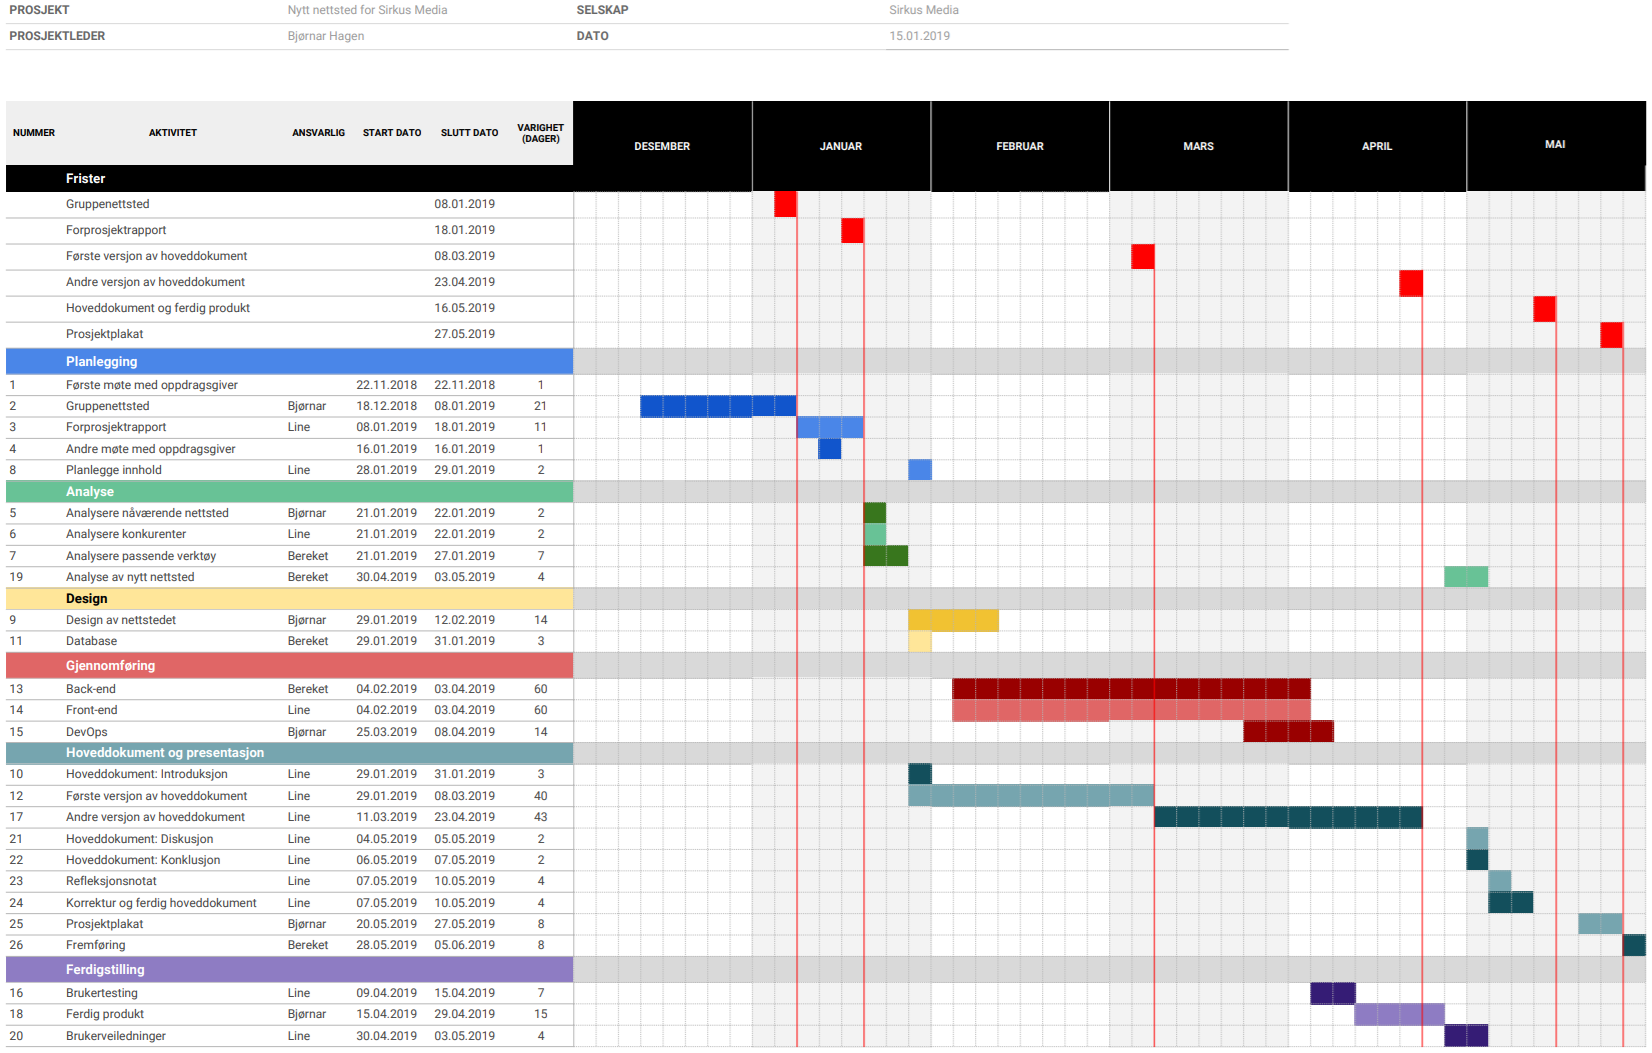
\includegraphics[width=0.95\paperwidth]{Ganttchart.png}}
    \caption{Gantt-diagram for prosjektplanen}
    \label{fig:gantt-diagram}
\end{figure}

\smallskip

\subsection*{Risikoanalyse}

Vi har analysert de kritiske faktorer og flaskehalser vi mener kan dukke opp i løpet av prosjektet, og utarbeidet en tabell med følgende risikoanalyse:

\begin{figure}[H]
    \centering
    \makebox[\textwidth]{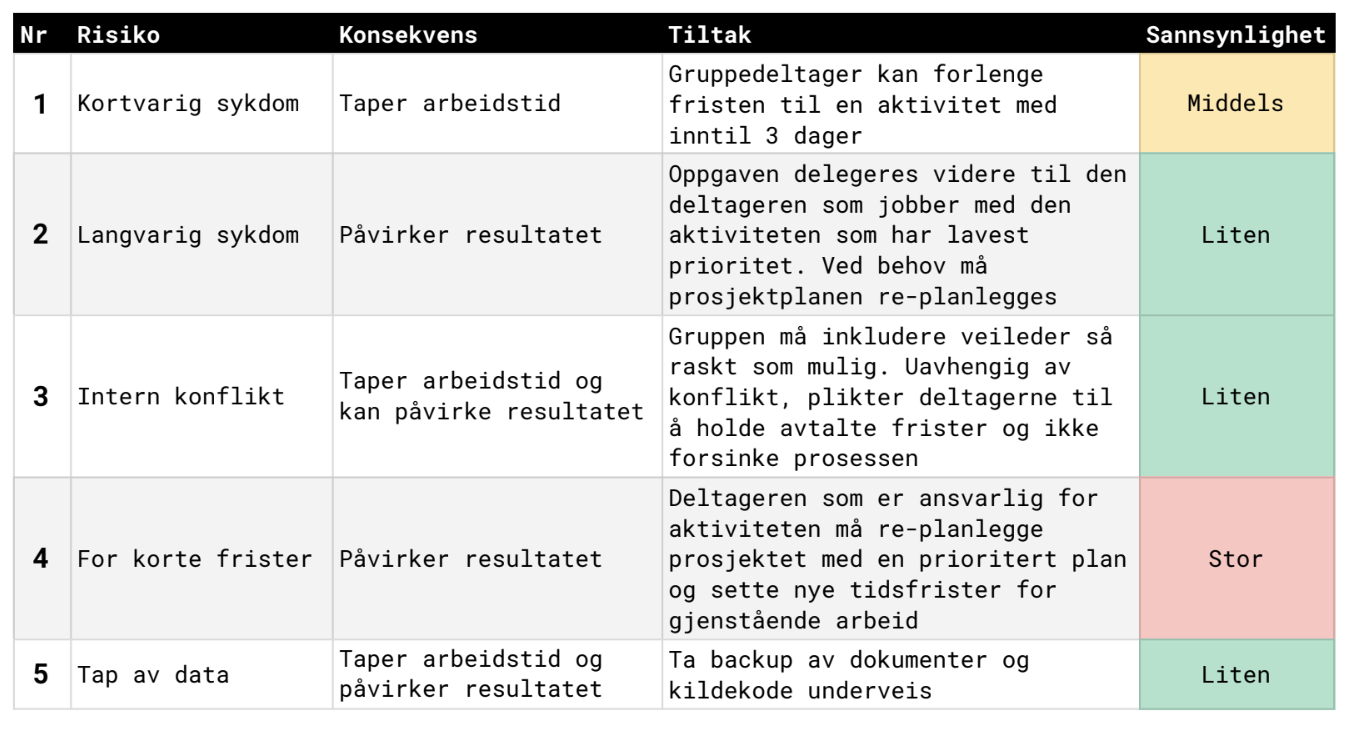
\includegraphics[width=0.90\paperwidth]{Risikoanalyse.png}}
    \caption{Risikoanalyse}
    \label{fig:risikoanalyse}
\end{figure}


\section*{Gjennomføring}

Medlemmene i gruppen plikter til å bidra like mye og skal delta med like mange timer. Medlemmene skal møtes minst en gang i uken for å jobbe sammen og oppgi status. Ved behov vil medlemmene møtes flere ganger i løpet av uken. I tillegg skal medlemmene ha fortløpende dialog via Facebook Messenger og Google Hangouts.


Det er besluttet å ha en fast prosjektleder, da det er nødvendig å ha en fast person som følger opp prosessen og som har ansvar for dialogen med både veileder og oppdragsgiver. Gruppen har vedtatt at personen som er best egnet til dette er Bjørnar.

Deltagerne har i tillegg fått hvert sitt overordnet ansvarsområdet når det kommer til gjennomføringen av nettstedet. Bereket har ansvar for back-end, Line for frond-end og Bjørnar for design og DevOps. Bjørnar vil også rullere mellom å jobbe med back-end og front-end, avhengig av behovet.

Versjonskontroll og backup av kildekode håndteres via Git. Deltagerne plikter å ta en sikkerhetkopi så fort man har opprettet og testet en ny kodebit. Selve prosjektstyringen skjer via en Kanban-tavle som er opprettet i Github. En aktivitet skal markeres som fullført så raskt som mulig av deltageren som utførte oppdraget. Gruppen følger en metodikk som ligner på Kanban-metodikken, men i dette prosjektet har deltagerne fått tildelt hver sin rolle. 

Gruppen skal ha fortløpende kontakt med oppdragsgiver, minimum etter hver fullførte aktivitet. Da har oppdragsgiver mulighet til å gi tilbakemelding underveis, slik at det ikke vil komme store endringer nær innlevering. Gruppen ønsker at tilbakemeldingene skal være skriftlige og ønsker hovedsaklig tilbakemeldinger på design og funksjonalitet. Dialogen med oppdragsgiver vil i hovedsak foregå over e-post, telefon og videosamtale. For slike type prosjekter er det ikke like stort behov for å ha møter fysisk, og gruppen vil få like stort utbytte gjennom videosamtaler. 

Deltagerne har avtalt å ha møter med veileder hver andre uke, som et minimum. Ved behov vil gruppen og veileder møtes hyppigere. Dette avtales med veileder over e-post.

\subsection*{Verktøy}

Oppdragsgiver har ikke satt krav til verken utforming, bruk av verktøy eller grafisk uttrykk. Vi har derfor fått ganske frie tøyler. Prosjektgruppen har følgelig selv valgt ut de forskjellige verktøyene vi mener passer bedriften og deres behov. Følgende verktøy vurderer vi i utgangspunktet å bruke:

\textit{Laravel}: et \textit{PHP} web-rammeverk som er basert på \textit{Symfony}. Det følger \textit{Model-view-controller} (MVC) designmønsteret. Dette skal vi bruke til å utvikle et \textit{REST-API} og vil fungere som \textit{back-end} til vårt nettsted.
\textit{React JS} er et \textit{JavaScript} bibliotek for å bygge brukergrensesnitt. Dette har vi tenkt å bruke som \textit{front-end} for vår løsning sammen med \textit{HTML} og \textit{CSS}. Før vi begynner å lage front-end har vi tenkt til å lage \textit{mockups} med \textit{Figma}.
For versjonskontroll har vi valgt å bruke \textit{Git}.
\textit{Repositories} lagres hos \textit{Github}, som vi også bruker for prosjektstyring. For  \textit{CI/CD} skal vi bruke \textit{Buddy.works}

Når nettstedet begynner å bli ferdig skal vi laste det opp på en server som kjører \textit{LEMP}-stacken (Linux, Nginx, MariaDB og PHP). Vi tenker å levere nettstedet over \textit{HTTP2}-protokollen, noe som gjør at vi trenger et \textit{SSL/TLS}-sertifikat for å servere nettsider over \textit{HTTPS}. Dette skaffer vi gjennom \textit{Let's Encrypt}. For å ta backup av databasen skal vi bruke \textit{Ottomatik.io}, og for backup av filer bruker vi \textit{AWS} (Amazon Web Services) sin \textit{S3} tjeneste, som vi også brukes for lagring av media-filer.

Når nettstedet er lansert skal vi måle trafikk og bruk av nettsidene ved hjelp av \textit{Google Analytics}.
\end{document}
